% Chapter Template

\chapter{Analysis of microscopy images to get network topology
parameters} % Main
% chapter title

\label{Chapter-Image} % Change X to a consecutive number; for referencing this
% chapter elsewhere, use \ref{ChapterX}

\lhead{Chapter 2. \emph{Analysis of microscopy images to get network topology
parameters}}
% Change X to a consecutive number; this is for the header on each page - perhaps a shortened title

%----------------------------------------------------------------------------------------
%	SECTION 1
%----------------------------------------------------------------------------------------
\section{Introduction}
\subsection{Image thresholding}
The gray levels of pixels belonging to an object are substantially
different from the gray levels of the background. Thresholding is way to
separate objects from the background.\\
\citet{sezgin_survey_2004} is a good review about the subject. The output of the
thresholding process is a binary image, whose one state will indicate the
foreground objects, while the complementary state will correspond to the
background.\\
\begin{equation}
P'_i=
   \begin{cases} 
     1               & \mbox{if } P_i > T   \\
     0               & \mbox{if } P_i < T
   \end{cases}
   \label{eq:bin}
\end{equation}
Where $P'_i\,\epsilon \, \{0{,} 1\}$ is the binarized output pixel , $P_i\,
\epsilon \,[0{,}255]$ is the gray-scale input pixel, and $T\,
\epsilon \,[0{,}255]$ is the threshold value.\\
  
There a lot of research in these filters, one of the most famous is the Otsu's
method, which is usually implemented by default in commercial software.
The Otsu's method minimizes the weighted sum of within-class variances of the
foreground and background pixels to establish an optimum threshold
\citep{sezgin_survey_2004}. This method belongs to the clustering-based methods
of thresholding. Further classification of thresholding is based on:
\begin{itemize}
  \item \textbf{Histogram shape.} Peaks, valleys and curvatures of the smoothed
  gray-level histogram are analyzed. \emph{Peak-and-valley}
  \item \textbf{Clustering.} The gray levels are clustered in two parts, one
  corresponding to the background and the other to the foreground. This method
  analyses separately each cluster. \emph{Otsu, Minimun error, fuzzy}.
  \item \textbf{Entropy.} Exploits the entropy of the distribution of the gray
  levels in the image. Maximization of entropy is indicative of high information transfer.
  Low cross-entropy between input gray level and output binary means
  preservation of information. \citet{pal_automatic_1983}
  were the first to use Shannon entropy in image analysis.
 \citep{pal_image_1988}
  \item \textbf{Object attribute.} Select the threshold based on some attribute
  quality between the original and binarized image. \emph{Edge matching, connectivity,
  shape compactness}.
  \item \textbf{Spatial methods}. This class not only uses the gray
  distribution, also studies the dependency of pixels in a neighborhood, for example, correlation
functions or co-ocurrence probabilities.
  \item \textbf{Local adaptive methods.} A threshold is calculated at each
  pixel, which depend on some local statistics, like \emph{variance}.
\end{itemize}

\begin{figure}[h]
\begin{center}
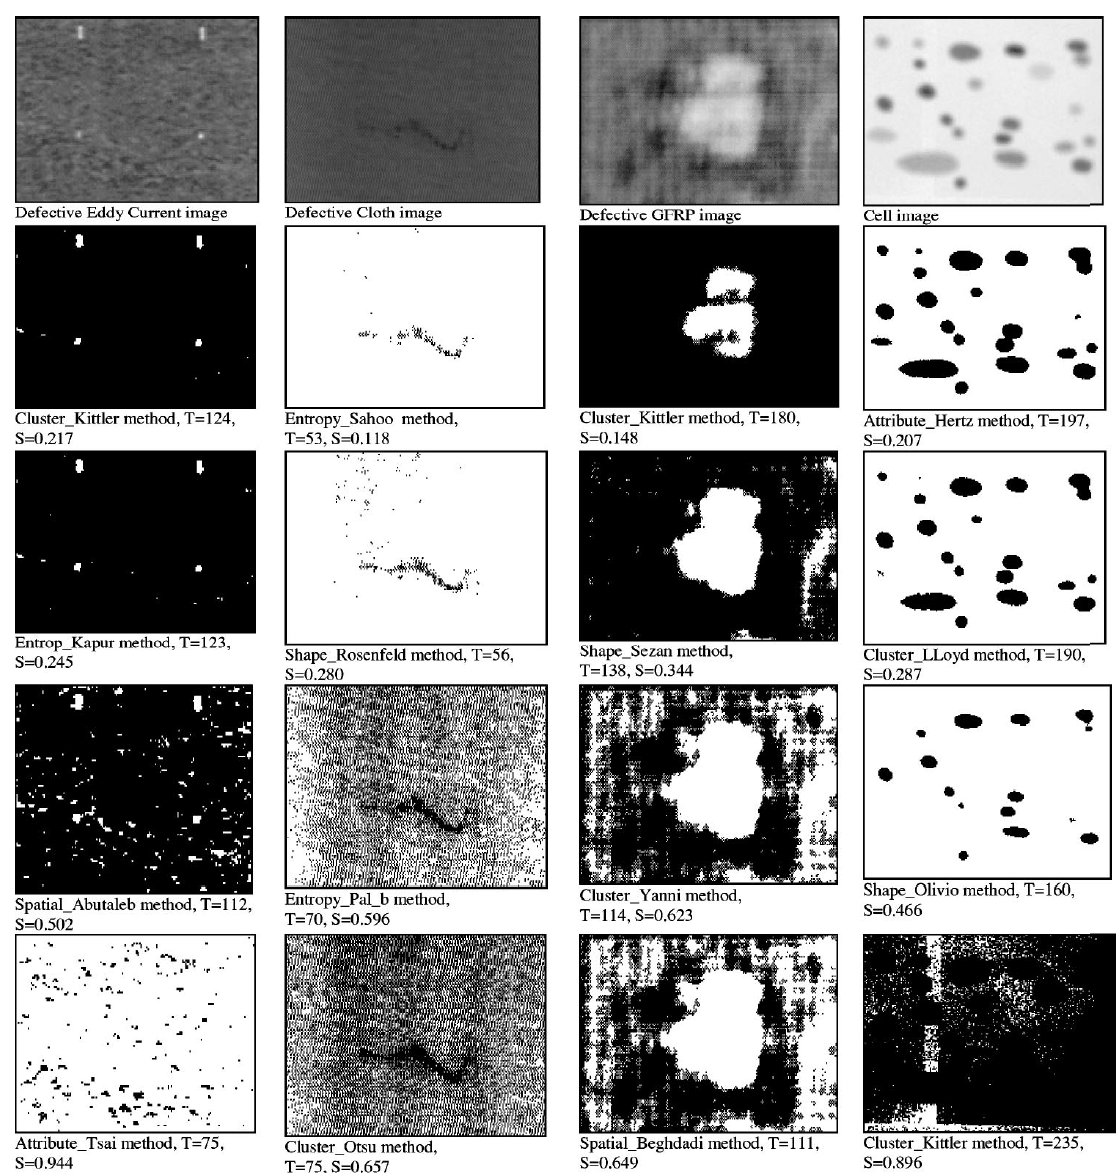
\includegraphics[width=0.9\textwidth,
height=0.6\textwidth]{Figures/fig_threshold_image.png}

\caption[Threshold calculation by different methods]{Different thresholding
results on sample images.\citep{sezgin_survey_2004}}
\label{fig:threshold}
\end{center}

\end{figure}

For our purposes, the binarization threshold will have an impact obtaining the
network. If the threshold is too high, long fibers will break in short,
unconnected pieces. If the threshold is too low, fibers that are clearly
separated, will become blurred together.\\
We have to choose the correct threshold that at the end of the process,
the processed image conserves the topology or architecture of the
original network. The unique way to do that is to rely in the best image
analyser that we have available, our brain . It seems straight forward to choose
the correct binarization threshold despite the initial complexity.
 
\begin{figure}[h]

\begin{minipage}{0.5\textwidth}
\subfloat[Input Image - Original]{%
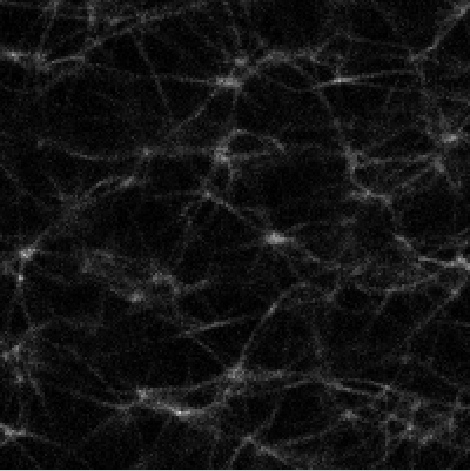
\includegraphics[width=0.9\textwidth]{Figures/binary/fig_bin_original.png}%
\label{original}}
\end{minipage}
\begin{minipage}{0.55\textwidth}
% \begin{minipage}{0.5\textwidth}
\subfloat[$T_P$=0.01]{%
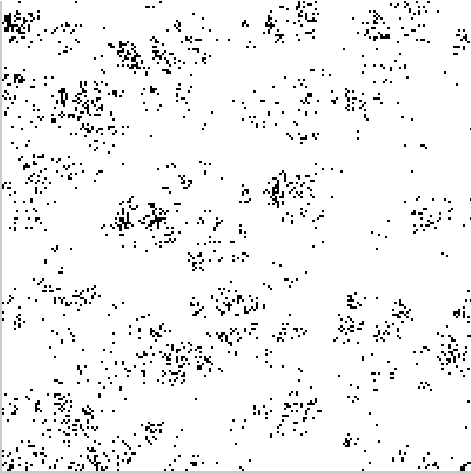
\includegraphics[width=0.45\textwidth]{Figures/binary/fig_bin_01.png}%
\label{001}}
\hspace{1pt}
\subfloat[$T_P$=0.08]{%
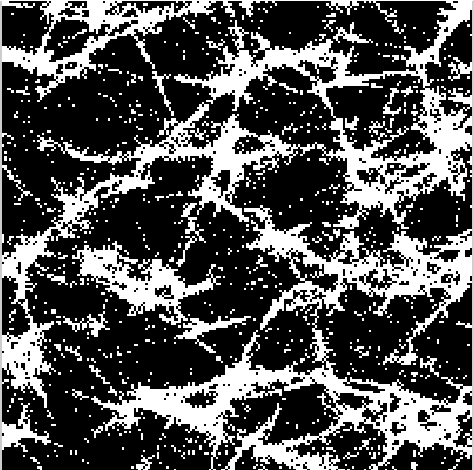
\includegraphics[width=0.45\textwidth]{Figures/binary/fig_bin_08.png}%
\label{008}}

\subfloat[$T_P$=0.1176]{%
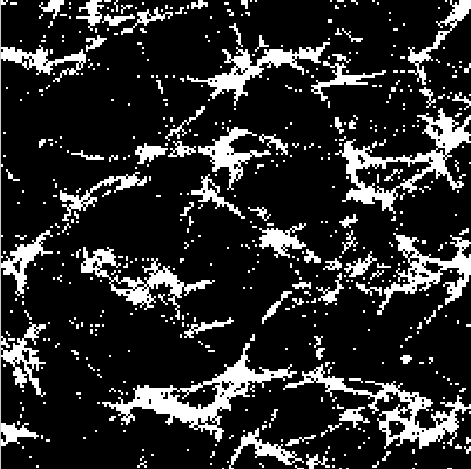
\includegraphics[width=0.45\textwidth]{Figures/binary/fig_bin_01176Otsu.png}%
\label{otsu}}
\hspace{1pt}
\subfloat[$T_P$=0.14]{%
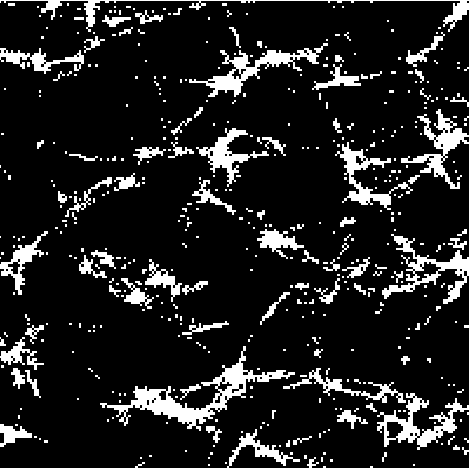
\includegraphics[width=0.45\textwidth]{Figures/binary/fig_bin_14.png}%
\label{014}}
\end{minipage}
% \\
% a)Original Image
% 
% % \end{subfigure}
% \\
% \begin{minipage}{0.5\textwidth}
% 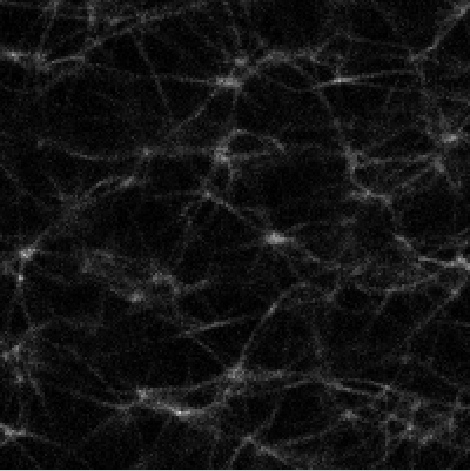
\includegraphics[width=0.3\textwidth]{Figures/binary/fig_bin_original.png}
% 
% \end{minipage}
\caption[Different threshold values on networks]{Different threshold values in
Actin network.
$T_P$ is the threshold value expressed as the percentage of the brightest pixel. If
$P_{max}$ is the brightest pixel, then $T=T_P\cdot P_{max}$. According to eq \ref{eq:bin}, any pixel greater than
that value is $1$ (white) at the output. At low values of threshold we have
blurred networks, at high values, connectivity information is lost.
\subref{otsu} corresponds to the threshold calculated by the Otsu's method }
\label{fig:binary}
\end{figure}

 
\section{FIbeR Extraction -FIRE- algorithm}

 I have used the algorithm from \citep{stein_algorithm_2008}. It is developed to
 analyze confocal stack of images. I have access to it after  Similar procedure.
 Note that in the future I would have to adapt this kind of algorithm to TEM
 tomography image stacks, where the $3D$ resolution might be worse. 
 \begin{description}
 \item[Smooth filter] Smooth the image with a Gaussian filter
 \item[Binarization threshold] Keep a percentage of the brightest pixels
 \item[Distance function- D] gfdgdfg
 
 \subitem \textbf{Smooth filter}
 \item[Nucleation points -NP-]
 \item[Local Maximum Points -LMP-]
 \end{description}
     
This analysis method \citep{stein_algorithm_2008} is based on a original idea of
\citet{wu_automated_2003}. Comparing both
algorithms, \citet{stein_algorithm_2008} main difference is the use of
multiple nucleation points and the restriction that each branch extend only in a single direction from a nucleation
point. In \citet{wu_automated_2003} the network has a single nucleation point 
at the global maximum of the distance function D.


%-----------------------------------
%	SUBSECTION 1
%-----------------------------------
\section{Skeletonization in Avizo}
The Avizo package XSkeleton. The access to Avizo is granted by a collaboration
with from Fonterra.

Step by step
 \begin{description}
 \item[Smooth filter] Smooth the image with a Gaussian filter
 \item[Binarization threshold] Multi-threshold module. This threshold is not
 based in percentage of the brightest pixel. It is a classical threshold turning
 to pure white $255$ or logical $1$ all pixels with a value greatest than the
 threshold value, and black $0$ all the pixels below that value.
 \item[Distance map] Distance map using Euclid distance. It assigns a value
 to each pixel equal to the distance from that pixel to the nearest black value. 
 \item[Thinner module] The module takes as input a label-field to be thinned and
 a distance map scalar field. It removes voxel by voxel from the segmented
 object until only a string of connected voxels remains.
 The thinning algorithm automatically detects dead end branches of skeleton
 spatial graphs. A parameter is used to distinguish them from noise on the
 interface  of the considered regions to avoid spurious branches.  Its default
 value is 5, i.e. the branches with a dead end which length is lower  than 5
 voxels are automatically considered as noise and removed.  Setting this to 10,
 which is a rather large value, leads to only a few branches remaining in the
 skeleton.  The drawback is that you also might miss real endpoints.
 
\item[Tace lines module] Converts an image that contains lines represented by
voxels into a spatial graph object.

 \end{description}

\begin{figure}[h]

% \begin{minipage}{0.5\textwidth}
 
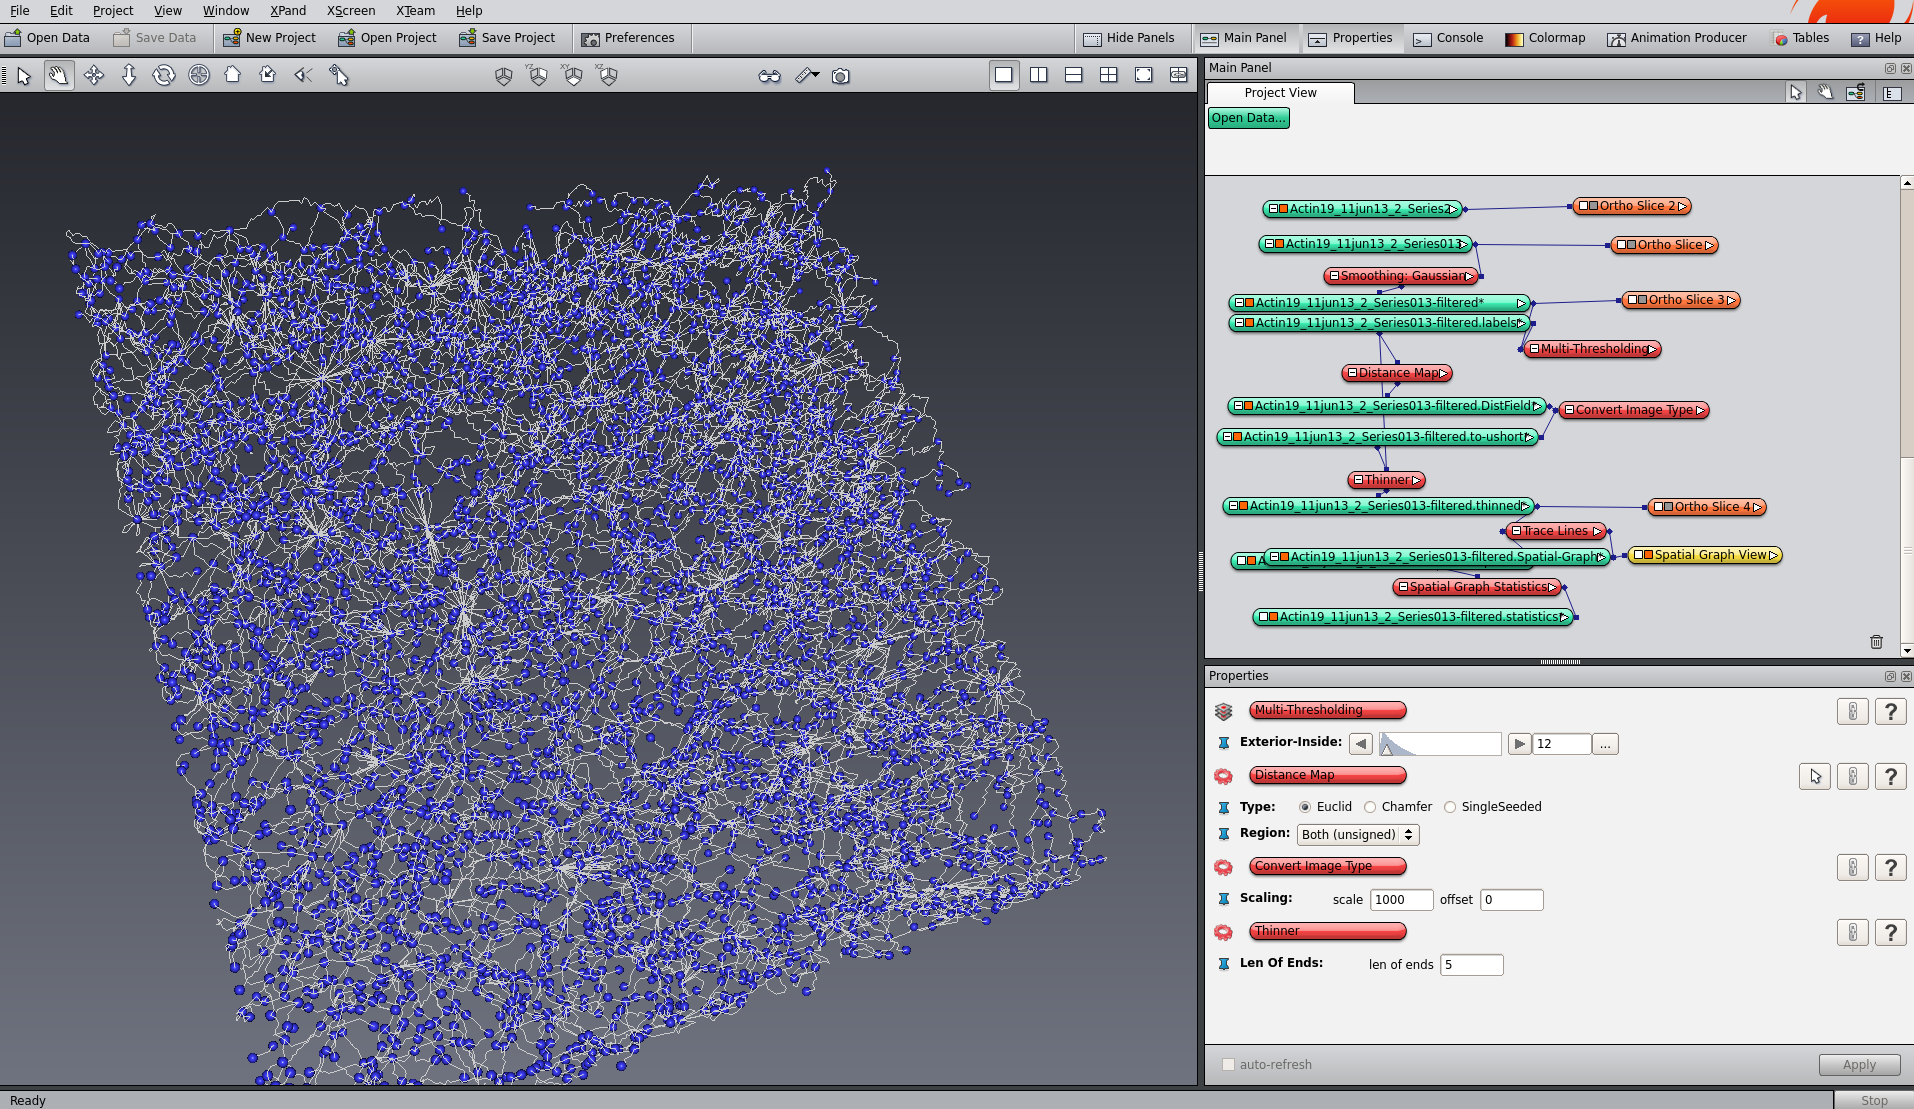
\includegraphics[width=1.1\textwidth]{Figures/avizoworkspaceactin.png}%

% \end{minipage}

% \\
% a)Original Image
% 
% % \end{subfigure}
% \\
% \begin{minipage}{0.5\textwidth}
% 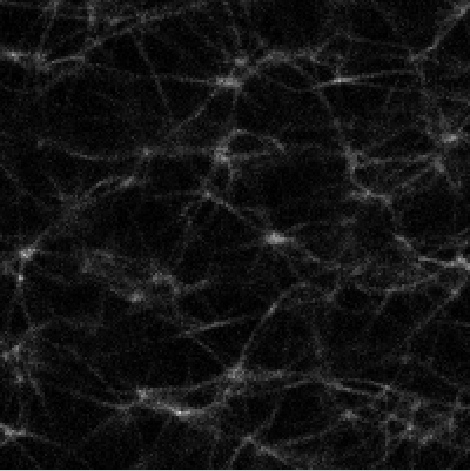
\includegraphics[width=0.3\textwidth]{Figures/binary/fig_bin_original.png}
% 
% \end{minipage}
\caption[Avizo image: Actin network visualization and workspace]{Avizo
workspace. Actin data visualization}
\label{fig:avizo_workspace}
\end{figure}

\section{Results}

Here we use 

